\chapter{Quantum Search}
The quantum search algorithm is another set of algorithms that can offer a speed up by using a quantum computer. It offers a speed-up of square root. Though it is not as great as the exponential speed up in case of quantum Fourier transform but still it is used for a large variety of problems and can offer speed up for the $NP$ problems.\\
The search problem may include a very large variety of problem. The normal search problems like searching for a number in a list of numbers can be said to have a structure. But the quantum search algorithm is much more general and can be used for larger variety of problems which may not even have a structure.
\subsection{Oracle}
For the search problem, we assume a very general structure. Let us say we have $N$ elements indexed from $0$ to $N-1$. Also we have a function $f(x)$ which verifies whether $x$ is a solution of the search problem or not i.e. it returns $1$ if $x$ is a solution otherwise it returns $0$. Note that $f(x)$ just verifies whether a given index is a solution of the search problem or not. It does not search for the solution. \\
We assume that we have a circuit which can implement the function $f(x)$. So, let us say that it is $O$. Then
\begin{equation}
O|x\rangle|y\rangle = |x\rangle |y \oplus f(x) \rangle
\end{equation}
\subsection{Solution(Grover's Algorithm)}
For the solution of quantum search problem, we need to apply the oracle described above repeatedly. Along with that we need one more operator which changes the phase of all the bases vector except the $|0\rangle$. So, it takes $|x\rangle$ to $-|x\rangle$ for all $x>0$. This can be written as $$P = 2|0\rangle \langle0| - I$$ Also, we need the number of solution $M$ but this can be calculated using phase estimation.\\
We take two registers- one is the output register and the second one is the oracle workspace register initialized to $(|0\rangle - |1\rangle) / \sqrt{2}$. The value of second register remains unchanged throughout the process. When we apply the oracle, the state is changed to $(-1)^{f(x)} |x\rangle (|0\rangle - |1\rangle )/\sqrt{2}$ and so only the phase of first register changes dependent on the value of $f(x)$.\\
We define the Grover operator as:
\begin{enumerate}
\item Apply the oracle O.
\item Apply $H$ on the first register.
\item Apply P gate on the first register.
\item Apply H gate again on the first register.
\end{enumerate}
The last three steps combine to give an operator $2|\psi\rangle \langle \psi | - I$ where $|\psi \rangle  = \sum |x\rangle$. This operator gives a flips the space about the $|\psi\rangle$ vector.\\
The first step flips the space about the space of vectors which are not the solutions of the search problem. In all, all the four steps shift the initial state towards the solution of the search problem. 
\begin{figure}[h]
\centering
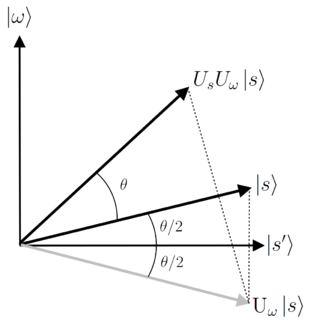
\includegraphics[width=0.75\textwidth]{images/grover.png}
\label{grover}
\caption{Phase diagram for Grover Iteration}
\end{figure}
\\In the above diagram, $|\omega\rangle$ is the space of the solution while $|s'\rangle$ is the space of other vectors. So, the state turns towards the solution by an angle $\theta$ given by:
\begin{equation}
cos(\theta/2) = \sqrt{\frac{(N-M)}{N}}
\end{equation}and after $k$ iterations of the Grover Algorithm
\begin{equation}
G^k|\psi \rangle  = \cos{\left(\frac{2k+1}{2}\theta\right)} |s' \rangle + \sin{\left(\frac{2k+1}{2}\theta\right)}|\omega \rangle
\end{equation}
So, the number of iterations before reaching the solution space is $k = \Bigg\lfloor\frac{ \arccos \sqrt{M/N}}{\theta} \Bigg\rfloor$.\\
Note that if the value of $M$ is greater than $N/2$, then the value of $k$ rises with $M$. So, we append extra $N$ numbers at the end which are not the solution to make it less than $N/2$.\\
$K$ is in the range of $O(\sqrt{N})$. So, we get a quadratic speedup in this case.\\
The circuit used is shown below:
\begin{figure}[h]
\centering
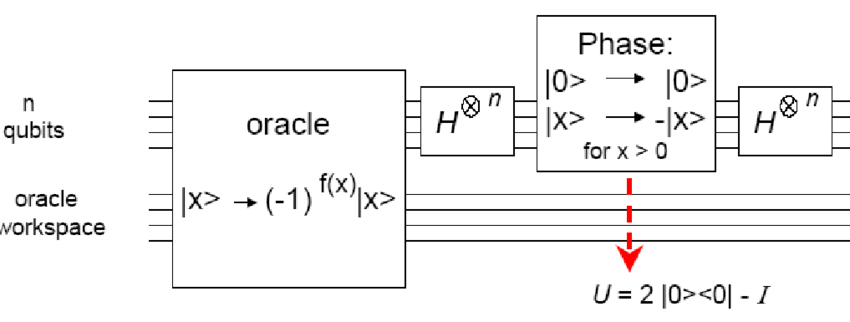
\includegraphics[width=1\textwidth]{images/grovercir.png}
\label{grovercir}
\caption{Circuit for Grover Iteration}
\end{figure}
\\The above circuit is repeated for $k$ number of times, to get the correct answer.
